\documentclass{beamer}

\usepackage{comment}
\usepackage{color}
\usepackage{listings}
\usepackage{verbatim}
\usepackage{multicol}
\usepackage{booktabs}
\definecolor{green}{RGB}{0,128,0}

\newcommand\gehcomment[1]{{{\color{orange} #1}}}
\newcommand\add[1]{{{\color{blue} #1}}}
\newcommand\remove[1]{\sout{{\color{red} #1}}}
\newcommand\codecomment[1]{{{\color{green} #1}}}
\newcommand\redcomment[1]{{{\color{red} #1}}}
\newcommand\bluecomment[1]{{{\color{blue} #1}}}
\newcommand\greencomment[1]{{{\color{green} #1}}}
\newcommand\magentacomment[1]{{{\color{magenta} #1}}}

\begin{comment}
\tiny
\scriptsize
\footnotesize
\small
\normalsize
\large
\Large
\LARGE
\huge
\Huge
\end{comment}

\begin{document}
\title{Geologic Disposal of Radioactive Waste}
\author{Emily Stein}
\date{\today}

%\frame{\titlepage}

%-----------------------------------------------------------------------------
\section{Titlepage}

\begin{frame}\frametitle{Geologic Disposal Safety Assessment}
These slides are part of PFLOTRAN primer - SAND2017-9449 TR
\end{frame}

%-----------------------------------------------------------------------------
\section{Location of Example}

\begin{frame}[fragile,containsverbatim]\frametitle{Location}

Location of this example problem:

\begin{semiverbatim}
> cd \$PFLOTRAN_DIR
> cd shortcourse/exercises/geologic_disposal
> ls
geologic_disposal.in
geologic_disposal.py
gdsa_usg.h5
hlw_heat.txt
metallic_heat.txt
obs_points.txt
obs_regions.txt
oxide_heat.txt
regions.txt
source_sink.txt
strata.txt
ufd-decay.dat
wfg.txt
\end{semiverbatim}

\end{frame}

%-----------------------------------------------------------------------------
\subsection{Command Line}
\begin{frame}[fragile]\frametitle{Command Line}
This problem might take a few minutes, so let's begin the simulation now.

\begin{itemize}
  \item Run the simulation
\end{itemize}

\begin{semiverbatim}
> cd \$PFLOTRAN_DIR
> cd shortcourse/exercises/geologic_disposal
> pflotran -input_prefix geologic_disposal
\end{semiverbatim}

\end{frame}

%-----------------------------------------------------------------------------
\section{Description of Geologic Disposal Scenario}

\subsection{Geologic Disposal Conceptual Model}

\begin{frame}\frametitle{Description of Geologic Disposal Scenario}
The ``Geologic Disposal Scenario'' demonstrates how to use the process models developed specifically for performance assessment simulations of deep geologic nuclear waste repositories, including \redcomment{WASTE\_FORM}, \redcomment{UFD\_DECAY}, and \redcomment{UFD\_BIOSPHERE}.
\begin{itemize}
  \item Problem domain: $3000 \times 5 \times 1005$ m (x $\times$ y $\times$ z)
  \item Grid resolution: 5/9 m to 15 m (unstructured grid)
  \item Flow mode: \redcomment{TH} (thermal/hydro)
  \item Heat Source: Function of time
  \item Radionuclide Sources: Defined with \redcomment{WASTE\_FORM}
  \item Radionuclide Behavior: Controlled by \redcomment{UFD\_DECAY}
  \item Dose: Calculated with \redcomment{UFD\_BIOSPHERE}
  \item Total simulation time: 500,000 y
\end{itemize}

\end{frame}

%-----------------------------------------------------------------------------
\frame{\frametitle{Geologic Disposal Schematic}
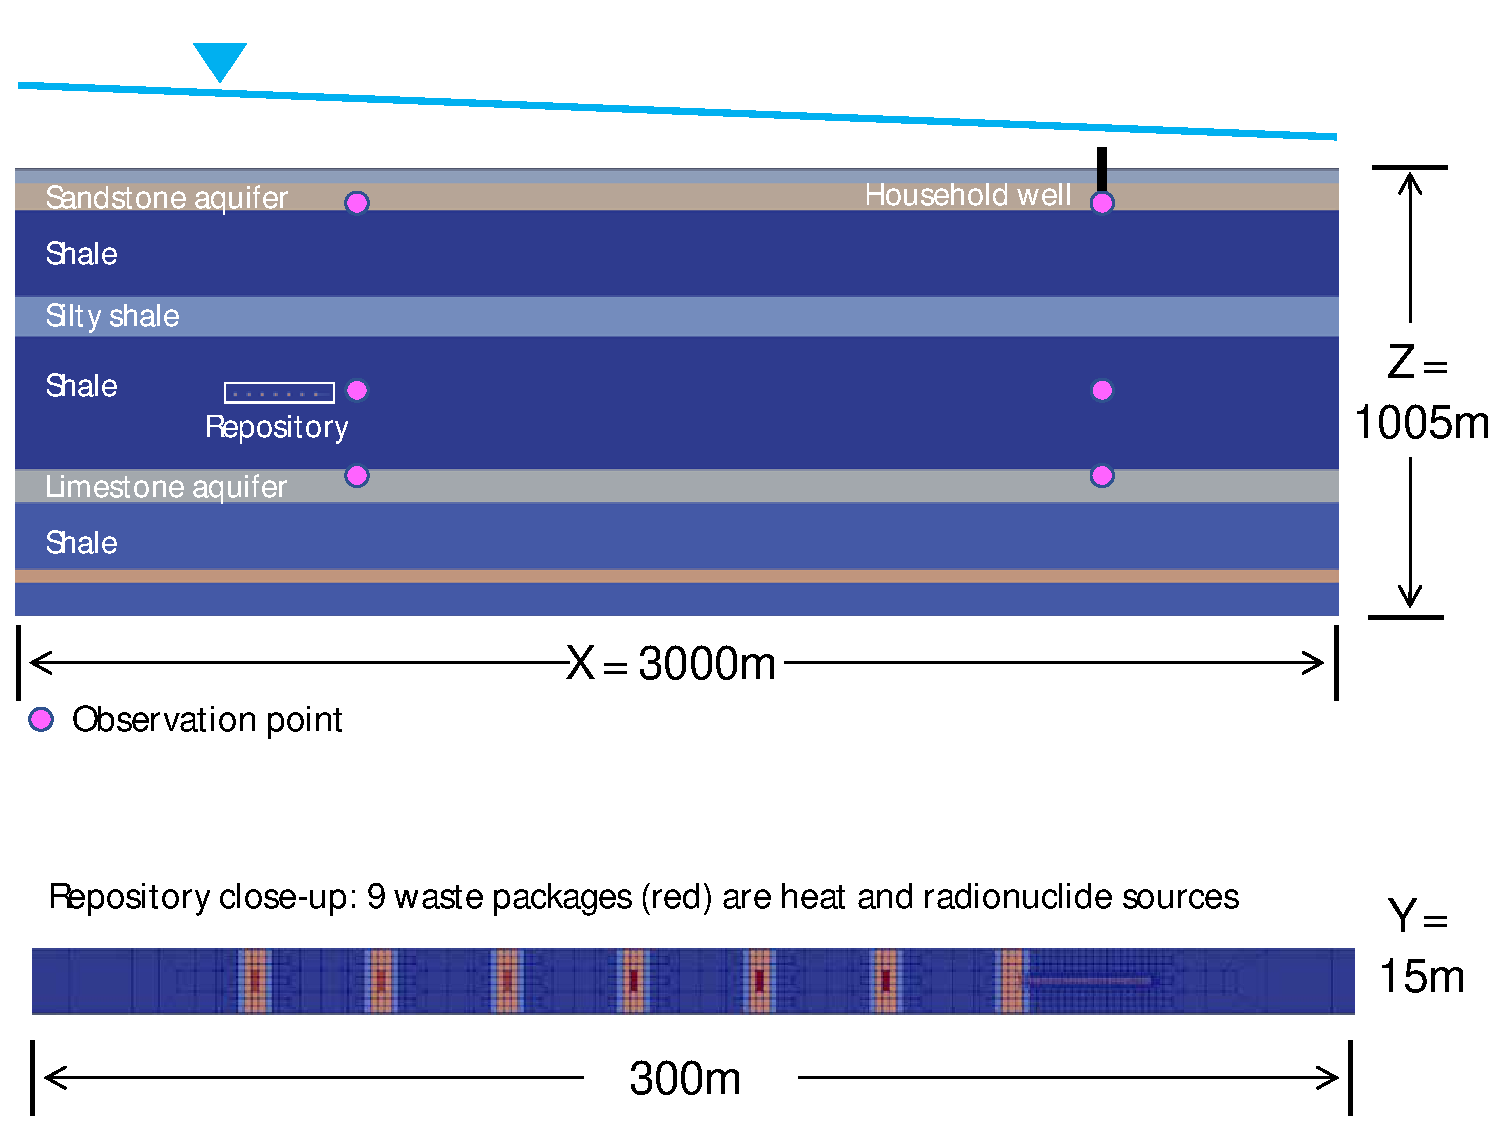
\includegraphics[width=\linewidth]{./gdsa_schematic}
}

%-----------------------------------------------------------------------------
\frame{\frametitle{Geologic Disposal Initial Conditions}
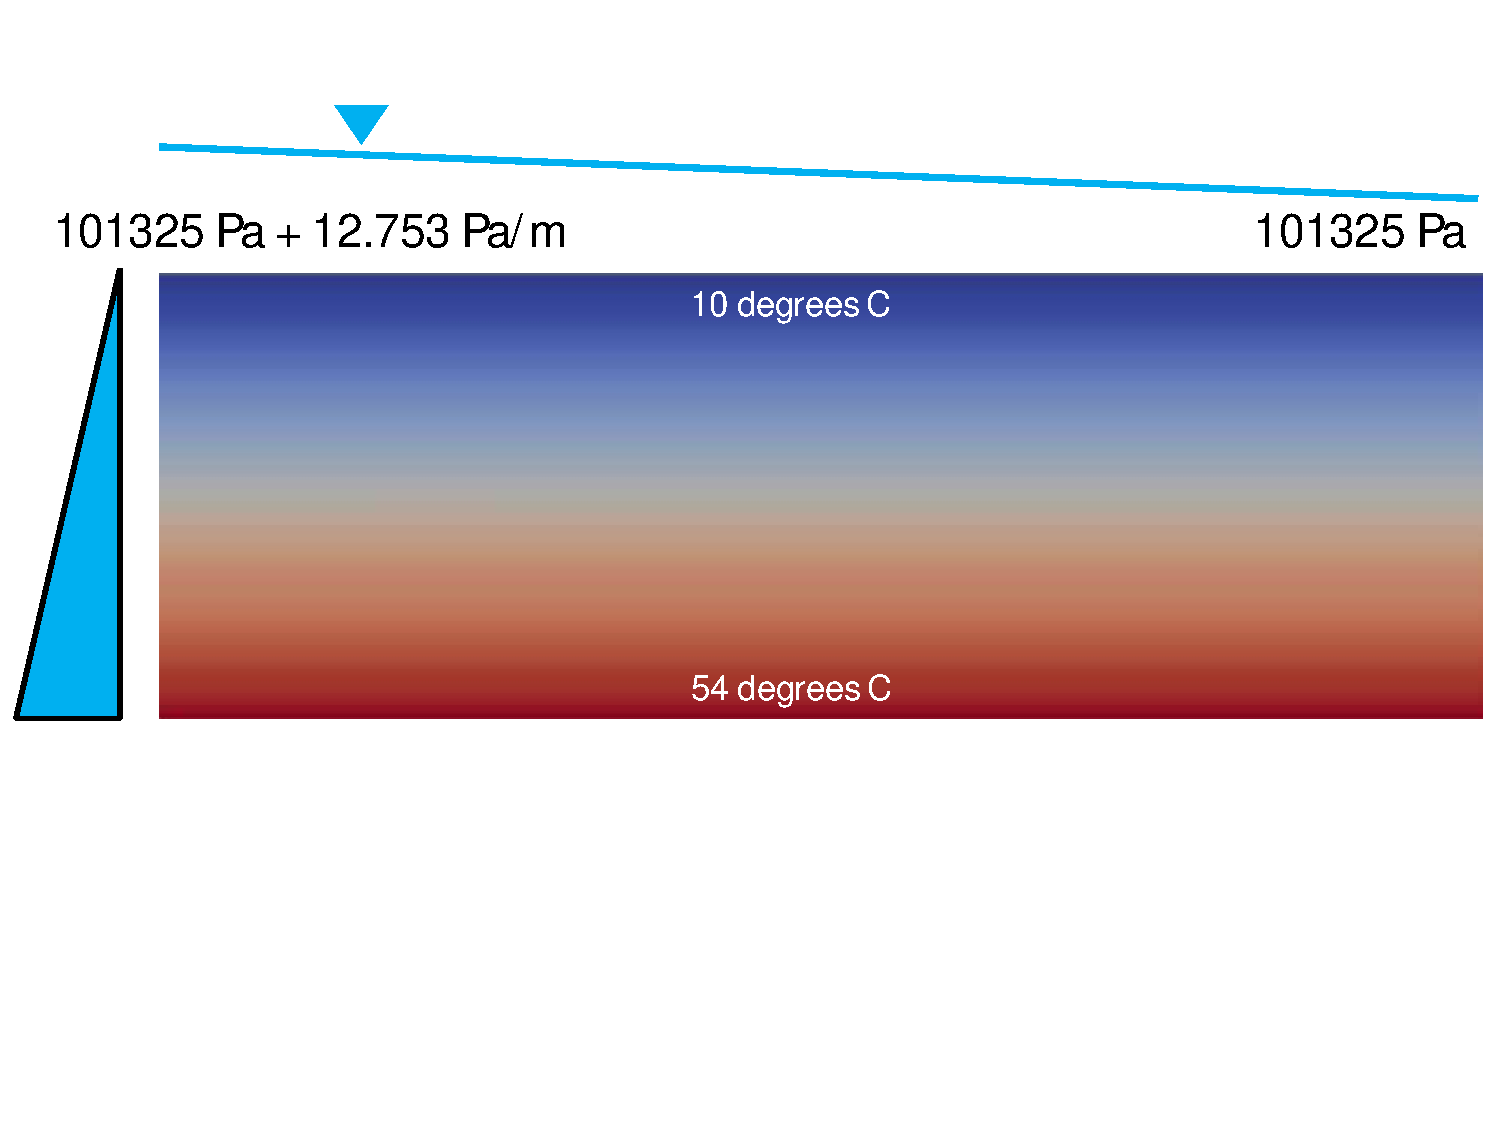
\includegraphics[width=\linewidth]{./gdsa_ic}
}

%-----------------------------------------------------------------------------
\section{Partial Description of Input Deck}

%-----------------------------------------------------------------------------
\subsection{SIMULATION}

\begin{frame}[fragile]\frametitle{SIMULATION}

\begin{semiverbatim}\small
SIMULATION
  SIMULATION_TYPE SUBSURFACE
  PROCESS_MODELS
    SUBSURFACE_FLOW flow
      MODE TH \bluecomment{! thermal/hydro}
    /   
    SUBSURFACE_TRANSPORT transport
      GLOBAL_IMPLICIT
    /
    UFD_DECAY ufd_decay \bluecomment{! in aqueous, solid, and sorbed phases}
    /
    WASTE_FORM wf_general \bluecomment{! waste package/form degradation}
    /
    UFD_BIOSPHERE bio \bluecomment{! dose calculation at a drinking well}
    /
  /
END
\end{semiverbatim}

\end{frame}

%-----------------------------------------------------------------------------
\subsection{DATASET}

\begin{frame}[fragile]\frametitle{DATASET}

\begin{itemize}
  \item Gridded datasets
  \item Used for initial and boundary conditions
\end{itemize}

\begin{semiverbatim}
DATASET 1d_temperature
  FILENAME ./initcond/reggrad0013.h5
  HDF5_DATASET_NAME hydrostatic_boundary_T
/
DATASET 1d_pressure
  FILENAME ./initcond/reggrad0013.h5
  HDF5_DATASET_NAME hydrostatic_boundary_P
/
\end{semiverbatim}

\end{frame}

%-----------------------------------------------------------------------------
\subsection{CHEMISTRY}

\begin{frame}[fragile]\frametitle{CHEMISTRY}

\begin{itemize}
  \item Aqueous and solid phase for each radionuclide
\end{itemize}

\begin{semiverbatim}
CHEMISTRY
  PRIMARY_SPECIES
    Am241
    Am243
    \bluecomment{...}
    I129
    Cs135
  /
  MINERALS
    Am241(s)
    Am243(s)
    \bluecomment{...}
    I129(s)
    Cs135(s)
  /
\end{semiverbatim}

\end{frame}

%-----------------------------------------------------------------------------
\begin{frame}[fragile]\frametitle{CHEMISTRY}

\begin{itemize}
  \item Rate constants = 0
\end{itemize}

\begin{semiverbatim}\small
  MINERAL_KINETICS
    Am241(s)
      RATE_CONSTANT 0.0d0
    /
    \bluecomment{...}
    Cs135(s)
      RATE_CONSTANT 0.0d0
    /
  /
  TRUNCATE_CONCENTRATION 1.d-21
  DATABASE ./ufd-decay.dat
  OUTPUT
    TOTAL \bluecomment{! aqueous concentration}
    ALL   \bluecomment{! all species}
  /
END
\end{semiverbatim}

\end{frame}

%-----------------------------------------------------------------------------
\subsection{GRID}

\begin{frame}[fragile]\frametitle{GRID}

\begin{itemize}
  \item Implicit \redcomment{unstructured} grid 
\end{itemize}

\begin{semiverbatim}
GRID
  TYPE UNSTRUCTURED ./gdsa_usg.h5
END
\end{semiverbatim}

\end{frame}

%-----------------------------------------------------------------------------
\subsection{EXTERNAL\_FILE}

\begin{frame}[fragile]\frametitle{EXTERNAL\_FILE}
\begin{itemize}
  \item Use the contents of another file in the input deck
\end{itemize}

\begin{semiverbatim}
EXTERNAL_FILE ./obs_points.txt \bluecomment{! OBSERVATION blocks}
\end{semiverbatim}

\begin{itemize}
  \item Elsewhere this input deck also contains:
\end{itemize}

\begin{semiverbatim}
EXTERNAL_FILE ./regions.txt \bluecomment{! REGION blocks}
EXTERNAL_FILE ./obs_regions.txt \bluecomment{! for OBSERVATION} 
EXTERNAL_FILE ./source_sink.txt \bluecomment{! heat SOURCE_SINK blocks}
EXTERNAL_FILE ./strata.txt \bluecomment{! STRATA blocks}
EXTERNAL_FILE ./wfg.txt \bluecomment{! WASTE_FORM blocks}
\end{semiverbatim}

\end{frame}

%-----------------------------------------------------------------------------
\subsection{FLOW\_CONDITION}

\begin{frame}[fragile]\frametitle{FLOW\_CONDITION}
\begin{itemize}
  \item{Using \redcomment{datasets}}
\end{itemize}

\begin{semiverbatim}
FLOW_CONDITION initial \bluecomment{! also for boundary conditions}
  TYPE
    PRESSURE DIRICHLET
    TEMPERATURE DIRICHLET
  /
  PRESSURE DATASET 1d_pressure
  TEMPERATURE DATASET 1d_temperature
END

\end{semiverbatim}
\end{frame}

\begin{frame}[fragile]\frametitle{FLOW\_CONDITION}
\begin{itemize}
  \item{1 of 3 heat \redcomment{sources} that change with time}
  \item{rates are specified in \greencomment{hlw\_heat.txt}}
\end{itemize}

\begin{semiverbatim}
FLOW_CONDITION hlw
  TYPE
    RATE MASS_RATE
    ENERGY_RATE SCALED_ENERGY_RATE VOLUME \bluecomment{! vol ave}
  /
  \bluecomment{!SYNC_TIMESTEP_WITH_UPDATE}
  INTERPOLATION LINEAR \bluecomment{! interpolate between times}
  RATE 0.d0 \bluecomment{! liquid flux rate}
  ENERGY_RATE FILE ./hlw_heat.txt \bluecomment{! list of times, watts}
END

\end{semiverbatim}
\end{frame}

\begin{frame}[fragile]\frametitle{FLOW\_CONDITION}
\begin{itemize}
  \item{\greencomment{hlw\_heat.txt}}
\end{itemize}

\begin{semiverbatim}\small
TIME_UNITS y
DATA_UNITS W
\bluecomment{! time energy (W/waste package)}
0.00E+00        1.755E+02
1.00E-01        1.751E+02
2.00E-01        1.747E+02
3.00E-01        1.743E+02
4.00E-01        1.739E+02
5.00E-01        1.735E+02
6.00E-01        1.732E+02
7.00E-01        1.728E+02
8.00E-01        1.724E+02
9.00E-01        1.720E+02
1.00E+00        1.716E+02
\bluecomment{...}
2.00E+05        6.631E-02
5.00E+05        6.488E-02
/
\end{semiverbatim}
\end{frame}

%-----------------------------------------------------------------------------
\subsection{END\_SUBSURFACE}
\begin{frame}[fragile]\frametitle{END\_SUBSURFACE}

\begin{itemize}
  \item Close the SUBSURFACE block
\end{itemize}

\begin{semiverbatim}
END_SUBSURFACE 

\bluecomment{! WASTE_FORM, UFD_DECAY, UFD_BIOSPHERE follow}
\end{semiverbatim}
\end{frame}

%-----------------------------------------------------------------------------
\subsection{WASTE\_FORM}
\begin{frame}[fragile]\frametitle{WASTE\_FORM GENERAL}

\begin{itemize}
  \item \redcomment{WASTE\_FORM} block for each waste package
  \item \redcomment{MECHANISM} block for each type of waste (next slide)
\end{itemize}

\begin{semiverbatim}\small
WASTE_FORM_GENERAL
  \bluecomment{! WASTE_FORM blocks are in} \greencomment{wfg.txt}
  EXTERNAL_FILE ./wfg.txt
  PRINT_MASS_BALANCE \bluecomment{! optional}
\end{semiverbatim}

\begin{itemize}\small
  \item Example \redcomment{WASTE\_FORM} block in \greencomment{wfg.txt}
\end{itemize}

\begin{semiverbatim}
  WASTE_FORM
     REGION hlw0              \bluecomment{! couple to a region}
     EXPOSURE_FACTOR 5.416057 \bluecomment{! adjust surface area}
     VOLUME 9.500000 \bluecomment{! m^3}
     MECHANISM_NAME hlw \bluecomment{! dissolution mech. & inventory}
  /
\end{semiverbatim}
\end{frame}

%-----------------------------------------------------------------------------
\subsection{WASTE\_FORM}
\begin{frame}[fragile]\frametitle{WASTE\_FORM GENERAL}

\begin{semiverbatim}\small
  MECHANISM GLASS
    KIENZLER_DISSOLUTION
    NAME hlw
    SPECIFIC_SURFACE_AREA 2.8d-3 m^2/kg
    MATRIX_DENSITY 2750. kg/m^3
    SPECIES
    \bluecomment{!r'n, atom wt (g/mol), 1/s, g/g, instant release, daughter}
      Am241  241.06d0  5.08d-11  3.179d-7  0.0d0  Np237
      Am243  243.06d0  2.98d-12  6.348d-10 0.0d0  Pu239
      \bluecomment{...}
       I129  128.90d0  1.29d-15  3.944d-8  0.0d0
      Cs135  134.91d0  9.55d-15  1.517d-5  0.0d0
    /
    CANISTER_DEGRADATION_MODEL
      VITALITY_LOG10_MEAN -4.5
      VITALITY_LOG10_STDEV 0.5
      VITALITY_UPPER_TRUNCATION -3.0
      CANISTER_MATERIAL_CONSTANT 1500.
    /
  END \bluecomment{! MECHANISM GLASS}

\end{semiverbatim}
\end{frame}
%-----------------------------------------------------------------------------
\subsection{UFD\_DECAY}
\begin{frame}[fragile]\frametitle{UFD\_DECAY}

\begin{itemize}
  \item \redcomment{Solubility} limits and \redcomment{sorption} coefficients for each element
\end{itemize}

\begin{semiverbatim}\small
UFD_DECAY
  ELEMENT Am
    SOLUBILITY 4.d-7 \bluecomment{! mol/L}
    KD \bluecomment{! kg water / m^3 bulk}
      metallic 0.d0
      hlw 0.d0
      oxide 0.d0
      buffer 2.11d7
      shale 1.08d8
      drz 1.08d8
      siltstone 1.08d8
      sandstone 2.17d5
      limestone 2.17d5
      lower_shale 1.08d8
      overburden 1.08d8
      lower_sandstone 2.17d5
    /
  /
\end{semiverbatim}
\end{frame}

\begin{frame}[fragile]\frametitle{UFD\_DECAY}

\begin{itemize}
  \item \redcomment{Decay rates} and \redcomment{daughters} for each isotope
\end{itemize}

\begin{semiverbatim}\small
  ISOTOPE Am241
    ELEMENT Am
    DECAY_RATE 5.08d-11 \bluecomment{! 1/s}
    DAUGHTER Np237 1.d0
  /
  ISOTOPE Am243
    ELEMENT Am
    DECAY_RATE 2.98d-12 \bluecomment{! 1/s}
    \bluecomment{!DAUGHTER Pu239 1.d0}
  /
\bluecomment{...}

END \bluecomment{! UFD_DECAY}
\end{semiverbatim}
\end{frame}

%-----------------------------------------------------------------------------
\subsection{UFD\_BIOSPHERE}
\begin{frame}[fragile]\frametitle{UFD\_BIOSPHERE}

\begin{itemize}
  \item Information about well and individual consumption
\end{itemize}

\begin{semiverbatim}\small
UFD_BIOSPHERE

skip \bluecomment{! not using this right now}
  ERB_1A A_model1 \bluecomment{! use this model with extraction}
    REGION well
    INDIVIDUAL_CONSUMPTION_RATE 2.d0 L/day
    \bluecomment{! INCLUDE_UNSUPPORTED_RADS}
  /
noskip \bluecomment{! end the skip statement}

  ERB_1B B_model1 \bluecomment{! use this model without extraction}
    REGION fake_well \bluecomment{! does not extract}
    DILUTION_FACTOR 1.0 \bluecomment{! use dilution factor instead}
    INDIVIDUAL_CONSUMPTION_RATE 2.d0 L/day
    \bluecomment{! INCLUDE_UNSUPPORTED_RADS}
  /

\end{semiverbatim}
\end{frame}

\begin{frame}[fragile]\frametitle{UFD\_BIOSPHERE}

\begin{itemize}
  \item Information about radionuclides
\end{itemize}

\begin{semiverbatim}\small
  SUPPORTED_RADIONUCLIDES
    RADIONUCLIDE I129
      ELEMENT_KD 0.d0  \bluecomment{! L-water/kg-solid}
      DECAY_RATE 1.40d-15 1/sec
      INGESTION_DOSE_COEF 1.1d-7 Sv/Bq
    /
    \bluecomment{...}
  /
  OUTPUT_START_TIME 1.d4 y
END \bluecomment{! UFD_BIOSPHERE}
\end{semiverbatim}
\end{frame}

%-----------------------------------------------------------------------------
\subsection{Command Line}
\begin{frame}[fragile]\frametitle{Command Line}

\begin{itemize}
  \item Plot the results
\end{itemize}

\begin{semiverbatim}
> python geologic_disposal.py
\end{semiverbatim}

\end{frame}

%-----------------------------------------------------------------------------
\end{document}
